\begin{flushleft}
	\textsl{It is a fact of sociology that topologists}\\
	\textsl{are interested in quadratic forms.}\\
	\rule[0pt]{17em}{0.5pt}\\
	\textsl{-- Serge Lang}
	\vspace{2em}
\end{flushleft}

The goal of this chapter is to construct

\begin{theorem}\label{thm:signature_8_existence_theorem}
	For any $t\in \Z$, there is a framed $4k$-manifold $M$ bounding a homotopy sphere and with signature $\sigma(M)=8t$.
\end{theorem}

Given a commutative coefficient ring $\Lambda$ and a $2m$-dimensional Poincar\'e pair $(X,Y)$, its intersection form is the bilinear form on middle dimensional cohomology
given by
\[ 
	\lkxfunc{Q_{X,Y}}{\H^m(X,Y; \Lambda)^{\times 2}_{\textrm{free}}}{\Lambda}{\omega, \eta}{(\omega\smile \eta)\frown [X,Y]}
\]
where $[X,Y]\in \H_m(X,Y; \Lambda)$ is a fundamental class and $\H^m(X,Y; \Lambda)_{\textrm{free}}$ denotes the free component of the $\Lambda$-module $\H^m(X,Y;\Lambda)$. 

\section{Intersection Theory}

\pagebreak

While the algebraic definition of the intersection form is useful for computation, there is a geometric way to interpret the data of the intersection form as actually counting the number of intersections between $m$-dimensional submanifolds in general position.

\subsection*{Compact Surfaces}

The simplest examples of the geometric data present in the intersection form occurs in the case of compact surfaces. Compact surfaces admit a succinct classification theorem:
\begin{theorem}[Classification of Compact Surfaces]
	Every closed $2$-manifold is homeomorphic to exactly one of the following 
	\[
			S^2,\quad \hash^p T^2, \quad \hash^q \RP^2,
	\]
	where $T^2=S^1\times S^1$ is the torus.
\end{theorem}

\begin{convention*}
The connected sum of a space $X$ with itself $n$ times will be denoted by $\#^n X$.
\end{convention*}

For the basic surfaces $S^2, T^2,$ and $\RP^2$, we have the cohomology rings
\[
		\begin{aligned}
			\H^\bullet(S^2; \Z_2) &= \Z_2[x]/(x^2)\quad &|x|=2,\\
			\H^\bullet(T^2; \Z_2) &= \Z_2[x,y]/(xy, x^2,y^2)\quad &|x|=|y|=1,\\
			\H^\bullet(\RP^2; \Z_2) &= \Z_2[x]/(x^3)\quad &|x|=1.\\
		\end{aligned}
\]
Correspondingly, the $\Z_2$-intersection forms can be written in matrix form as
\[
	Q_{S^2} = \begin{bmatrix}0\end{bmatrix}, \quad Q_{T^2} = \begin{bmatrix}0&1\\ 1&0\end{bmatrix}, \quad Q_{\RP^2} = \begin{bmatrix}1\end{bmatrix}.
\]
This represents 

\begin{theorem}[Classification of Compact Surfaces]
	The intersection form is an isomorphism between the monoid of homeomorphism classes of compact surfaces under connected sum and the monoid of unimodular bilinear forms over $\Z_2$.
	\[
		\mathrm{Surf} \lkxto[Q] \mathrm{Bil}(\Z_2)
	\]
	Both monoids have presentation $\langle A,B \mid A+B = 3A\rangle$.
\end{theorem}

\subsection*{Intersections}

\begin{theorem}
	Suppose $M$ and $N$ are compact oriented submanifolds of dimensions $p$ and $q$ oof a compact oriented $n$-manifold $X$ with boundary such that $p+q=n$. Suppose they intersect transversally. Letting $\omega,\eta$ be the Poincar\'e duals to the fundamental classes $[M]\in \H_p(X)$ and $[N]\in \H_q(X)$, we have
	\[
		 Q_X(\omega, \eta) = \sum_{x\in M\cap N} \sgn(x).
	\]
\end{theorem}

\section{Integral Bilinear Forms}

\subsection*{Bilinear Forms and Matrices}

Let $M_n(R)$ be the ring of $n\times n$ matrices taking values in $R$. A matrix $Q\in M_n(R)$ is invertible if it's determinant $\det Q\in R$ is a unit, and we denote the group of invertible $n\times n$ matrices by $\GL_n(R)$. Two matrices $Q$ and $P$ are said to be conjugate if $P = \Lambda^\intercal Q\Lambda$ for some invertible matrix $\Lambda\in \GL_n(R)$. If we have a free $R$-module $M$ of rank $n$ with some basis $\{e_1,\ldots, e_n\}$, any matrix $Q\in M_n(R)$ defines a bilinear form on $M$ by
\[
	Q(v,w) = v^\intercal Q w\quad \textrm{for all }v,w\in M.
\]
We abuse notation by referring to the matrix and the form interchangeably.
Note that the bilinear form only depends on the matrix conjugacy class, and the form is independent of the basis for $M$.
Similarly, if we have a bilinear form on $M$, we can define the matrix $Q$ in some basis $\{e_1,\ldots, e_n\}\subset R^n$ by setting $Q_{ij}= Q(e_i, e_j)$.

In this way, many notions pertaining to matrices are mapped to notions pertaining to bilinear forms. For instance, symmetric matrices correspond to symmetric bilinear forms and skew-symmetric matrices correspond to skew-symmetric bilinear forms.

\begin{definition}
	A bilinear form $Q$ is said to be \defn{non-degenerate}[non-degenerate bilinear form] if its matrix has non-zero determinant. Equivalently, the form $Q$ is \defn{degenerate}[degenerate bilinear form] if there is some non-zero $v\in M$ such that
	\[Q(v,w)=0 \quad\quad \textrm{for all }w\in M.\]
\end{definition}

When working with rings $R$ which aren't fields, we can get a stronger notion of non-degeneracy if we require the determinant to not only be non-zero but also invertible in $R$.

\begin{definition}
	A bilinear form $Q$ is said to be \defn{unimodular} if its matrix is $R$-invertible. Sometimes, we also refer to an $R$-invertible matrix as unimodular if it is $R$-invertible.
\end{definition}

Equivalently, a bilinear form $Q$ is unimodular if the map
\[
	\lkxfunc{}{M}{M^\d}{v}{\left\{w\mapsto Q(v,w)\right\}}
\]
is an isomorphism. The condition for non-degeneracy only requires that this map be injective.

\begin{example}
	For instance, when $M=\Z$ as a $\Z$-module, the bilinear form $B(x,y)=2xy$ is non-degenerate but not unimodular.
\end{example}

\subsection*{Hasse-Minkowski Classification}

\begin{proposition}
	There is an even positive-definite unimodular form of rank $8$ corresponding to the matrix
	\[
		E_8 = \begin{pmatrix}
			2 & 1 &   &   &   &   &   &   \\
			1 & 2 & 1 &   &   &   &   &   \\
			  & 1 & 2 & 1 &   &   &   &   \\
			  &   & 1 & 2 & 1 &   &   &   \\
			  &   &   & 1 & 2 & 1 & 0 & 1 \\
			  &   &   &   & 1 & 2 & 1 & 0 \\
			  &   &   &   & 0 & 1 & 2 & 0 \\
			  &   &   &   & 1 & 0 & 0 & 2 \\
		\end{pmatrix}
	\]
\end{proposition}

\subsection*{Dodecahedral Space}

We know that there are no exotic spheres in dimension $3$, but what happens if we repeat the $\E_8$-plumbing construction in $4$-dimensions? While the boundary of the resulting manifold is not an exotic sphere, it has the homology of a $3$-sphere yet is not homeomorphic to the standard $3$-sphere.
This $3$-manifold is known as (Poincar\'e) \defn{dodecahedral space} and has a beautiful geometric construction. We'll denote this space by $\mathscr{D}$. Aside from being a wonderful example of a non-Euclidean geometry, this space also was the first counter-example to an incorrect earlier form of the Poincar\'e hypothesised which stated that every homology $3$-sphere was also homeomorphic to the $3$-sphere. Much like exotic spheres are counter-examples to the smooth Poincar\'e hypothesis, in a similar vein the dodecahedral space can be thought of as a sort of ``proto exotic sphere'' serving as a counter-example to the ``proto Poincar\'e hypothesis''.

The classic construction of dodecahedral space $\mathscr{D}$ is due to Poincar\'e \todo{cite}. We begin by letting $\mathcal{D}\subset \R^3$ be a solid dodecahedron in three dimensional Euclidean space. The dodecahedron has 6 pairs of opposite pentagonal faces. Picking a clockwise spherical orientation on $\mathcal{D}$, we can glue together opposing faces with a minimal clockwise twist to line them up (see \cref{fig:dodecahedral_space_construction}). The resulting quotient space is a closed $3$-manifold, and this manifold is dodecahedral space $\mathscr{D}$.

\begin{figure}[ht]
	\centering
	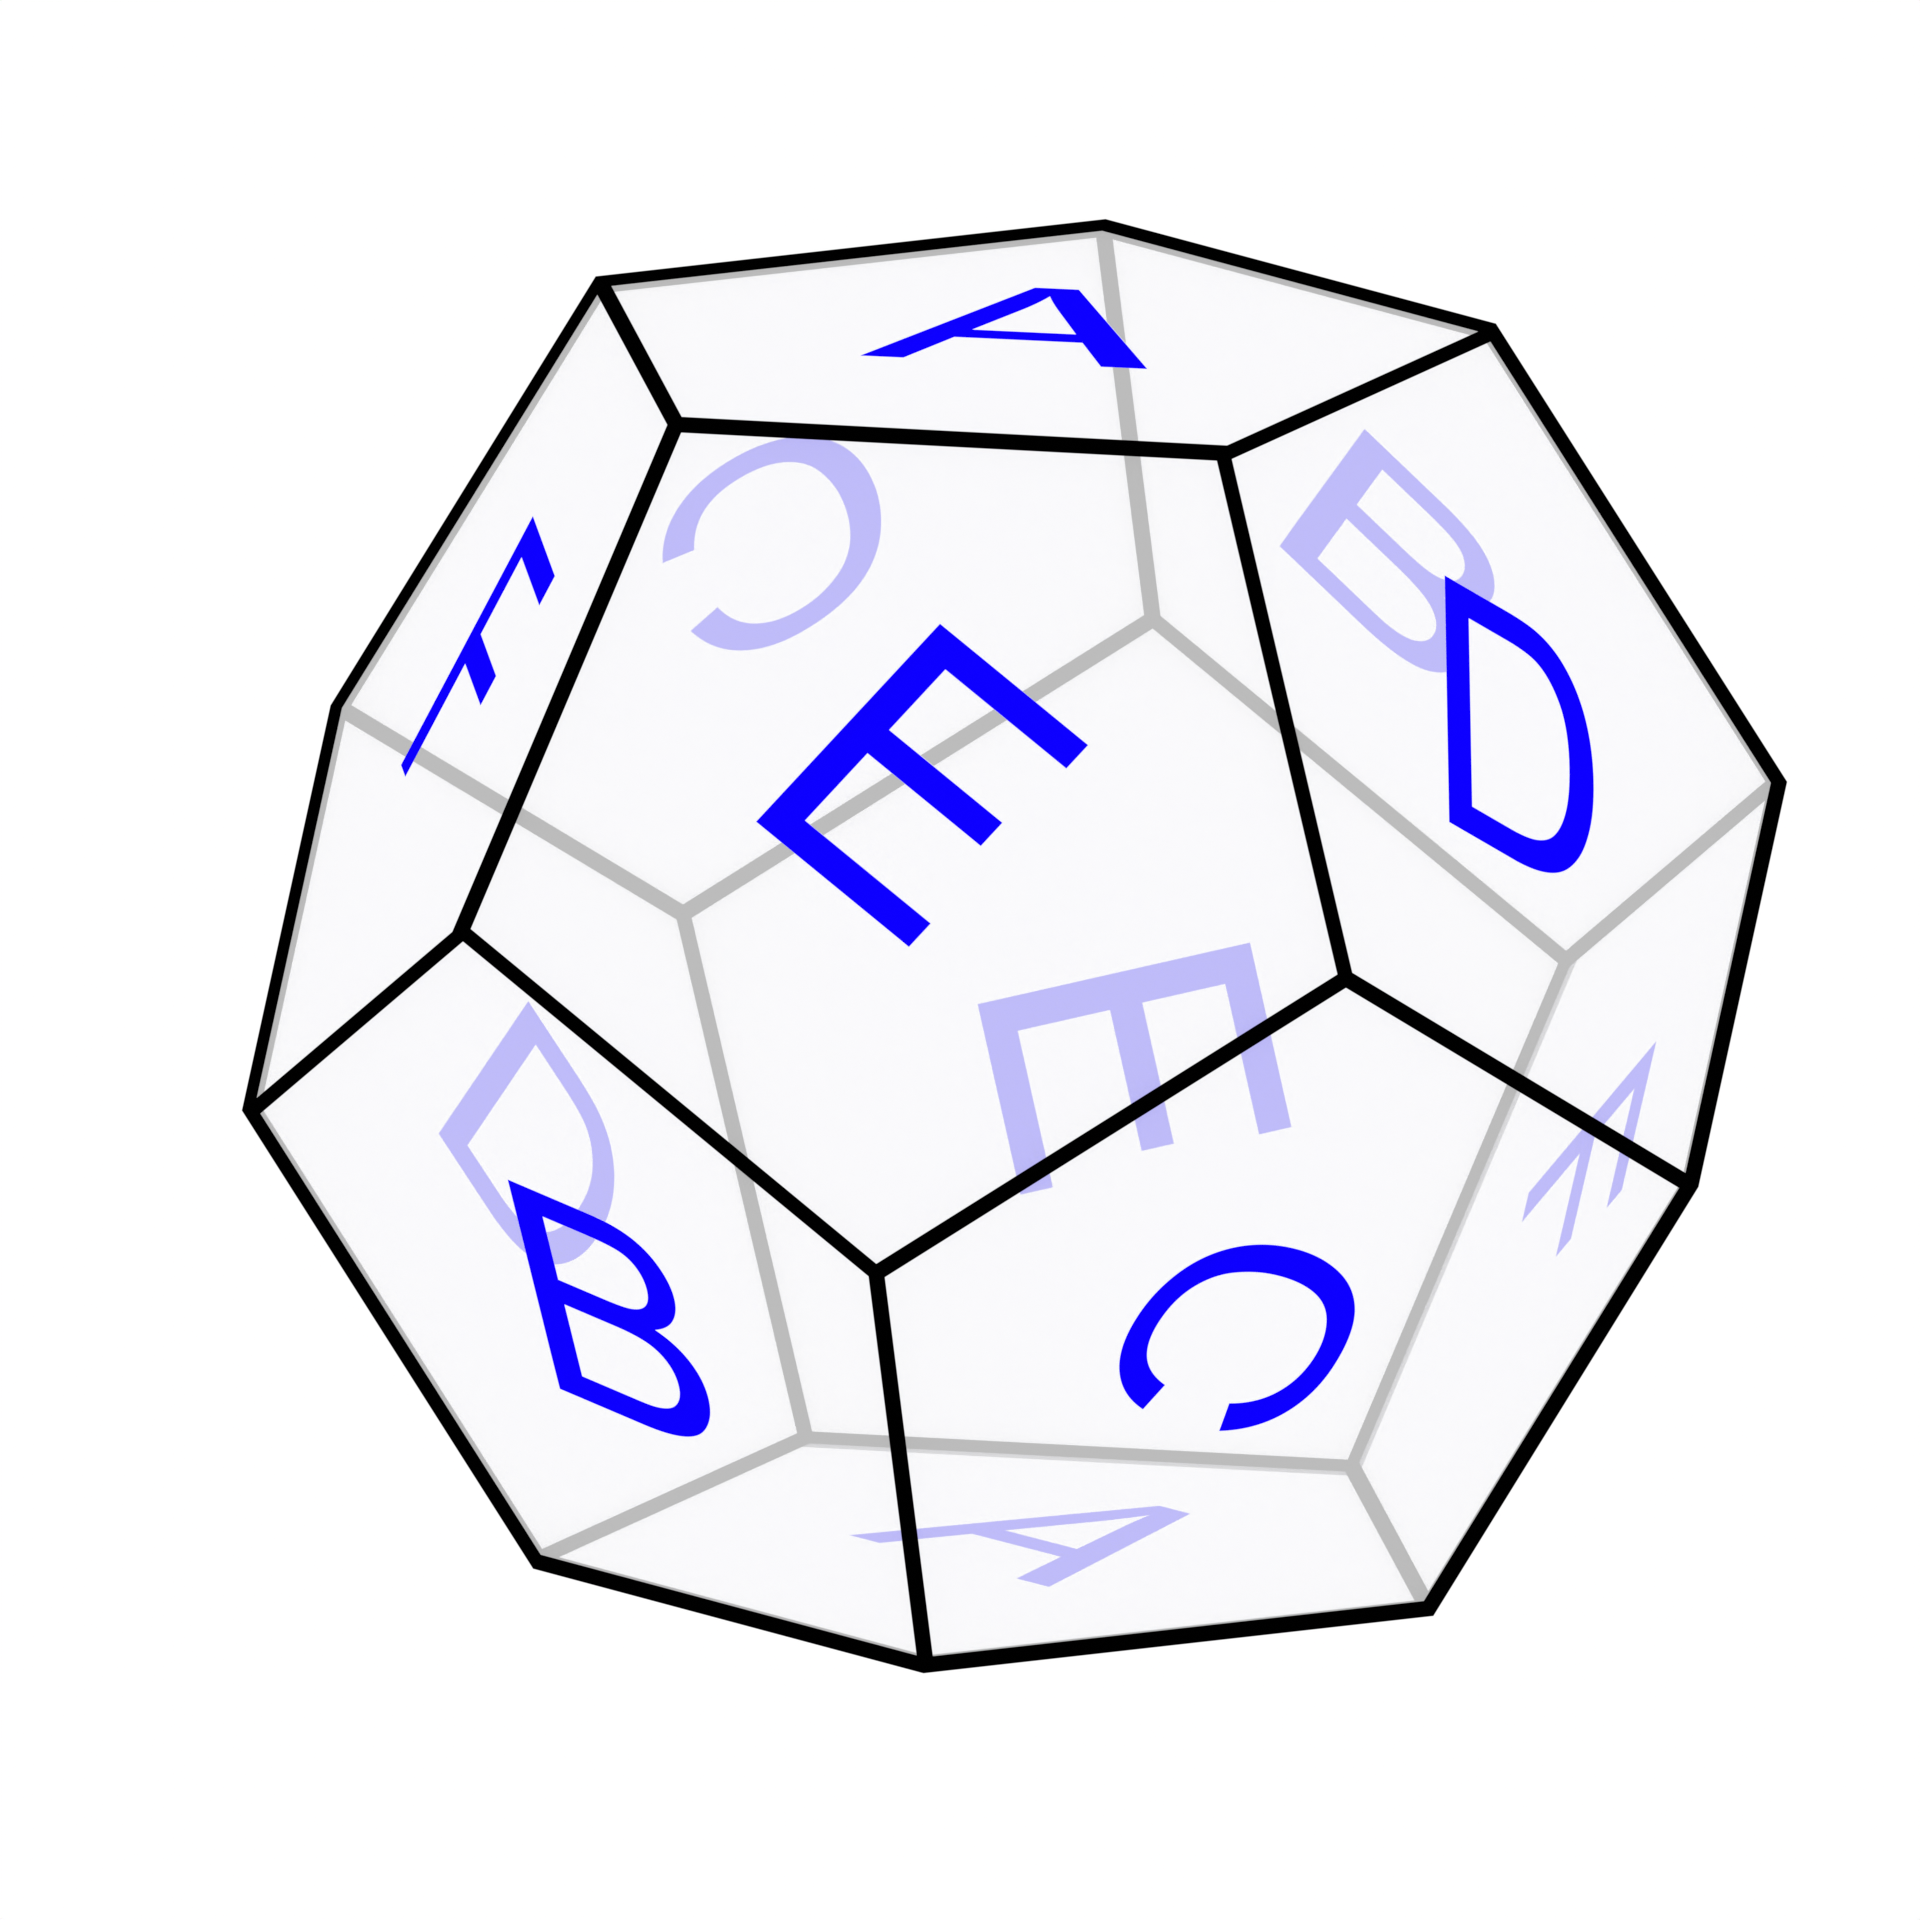
\includegraphics[width=2in]{graphics/temp-diagrams/dodecahedral-space-geometric-construction.png}
	\caption{Construction of Dodecahedral Space}\label{fig:dodecahedral_space_construction}
\end{figure}

Given this geometric construction, it should be fairly straightforward -- albeit tedious -- to compute the homology of dodecahedral space by means of a cellular decomposition. After such a computation, we would find that:
\begin{proposition}
	Dodecahedral space is a homology $3$-sphere.
\end{proposition}

While the first homology of dodecahedral space is trivial and incapable of differentiating dodecahedral space from a 3-sphere, the fundamental group reveals a much richer geometric structure. If we let $\SO_3$ act on $\R^3$ in the usual way, we can form the symmetry group $\Sym(\mathcal{D})\subset \SO_3$ of orientation preserving orthogonal transformations which leave the dodecahedron $\mathcal{D}$ unchanged. This is known as the \defn{icosahedral group}\footnote{The icosahedron and dodecahedron are dual, so the choice of icosahedral in the name is purely a historical convention.} $\mathrm{I}\subset \SO_3$, a group containing $60$ elements and isomorphic to the alternating group $A_5$. There is a double cover of $\SO_3$ by the $\Spin_3$ Lie group:
\[
	\SU_2\cong \Spin_3\lkxto[2:1] \SO_3
\]
The \defn{binary icosahedral group}, denoted $2\mathrm{I}$, is the preimage of $\mathrm{I}$ under this double cover and hence contains $120$ elements. Since there is an exceptional isomorphism $\SU_2\cong \Spin_3$, the binary icosahedral group admits a representation by unitary complex $2\times 2$ matrices.
We then have:
\begin{proposition}
	The fundamental group of dodecahedral space is the binary icosahedral group.
\end{proposition}
This hints at another interesting fact about the binary icosahedral group -- it is a \defn{perfect group}, which means that it's commutator subgroup is the entire group. By the Hurewicz isomorphism, it would follow that
\[
	\H_1(\mathscr{D}) \cong \Ab\left[ \pi_1(\mathscr{D})\right] \cong 2\mathrm{I}/[2\mathrm{I}, 2\mathrm{I}] = 0
\]
where $\Ab$ denotes the abelianization. This perfectness of the fundamental group thus ``hides'' the non-trivial topology of $\mathscr{D}$ from being detectable by homology. It's interesting to note that dodecahedral space and $S^3$ are the only homology $3$-spheres up to homeomorphism with finite fundamental groups.

There is also a useful construction of dodecahedral space which will later appear in our later study of Brieskorn manifolds in \cref{sec:brieskorn-manifolds}. If we identify $\SU_2$ with the $3$-sphere of unit quaternions, we obtain the construction:

\begin{proposition}
	There is a diffeomorphism $\mathscr{D} \cong S^3 / 2\mathrm{I}$ expressing dodecahedral space as the quotient of the $3$-sphere under a proper group action by $2\mathrm{I}$.
\end{proposition}

Finally, let's see how the dodecahedral space and binary icosahedral group arises out of the plumbing construction we've worked with thus far.

\todo{write this section}

\begin{proposition}
	There is a diffeomorphism $\mathscr{D}\cong \partial P^4(\E_8)$.
\end{proposition}

\todo{citations}

\begin{remark}
	In the early 2000's, the Wilkinson Microwave Anisotropy Probe (WMAP) was launched to accurately map out the cosmic microwave background, i.e. leftover heat from the Big Bang. The observed lack of temperature correlations above 60$^\circ$ led astrophysicist Jean-Paul Luminet to propose a cosmological model \cite{luminet2003dodecahedral} where the shape of the universe is a dodecahedral space, explaining the lack of large scale correlations by means of the compact topology of space. In such a finite universe, larger temperature correlations simply wouldn't have enough room to form.
	While this model made some predictions aligning with observed cosmological data
	\cite{roukema2008dodecahedral}, higher resolution data by the later Planck spacecraft later seemed to suggest that the observable large scale topology is trivial, leading to the modern prevalence of the $\Lambda$CDM model as a standard model for cosmology.
\end{remark}
